% Niveau :      PCSI *
% Discipline :  Chimie Orga
% Mots clés :   Stéréochimie

\begin{exercise}{Spectre RMN des acides aminés}{2}{PCSI}
{Chimie organique I,Spectroscopie,RMN}{bermu}

\begin{questions}
\questioncours Couplage spin-spin $^{2}J$, $^{3}J$ et $^{4}J$ en RMN du proton $^{1}$H. \\
On prendra soin d'expliquer l'origine du phénomène sur un exemple simple et d'énoncer des facteurs d'influence de la valeur de $J$.

\begin{EnvUplevel}
    Un$\cdot$e étudiant$\cdot$e de chimie a synthétisé le composé ci-dessous mais a trouvé étrange le spectre RMN qu'elle a obtenu :
    
    \noindent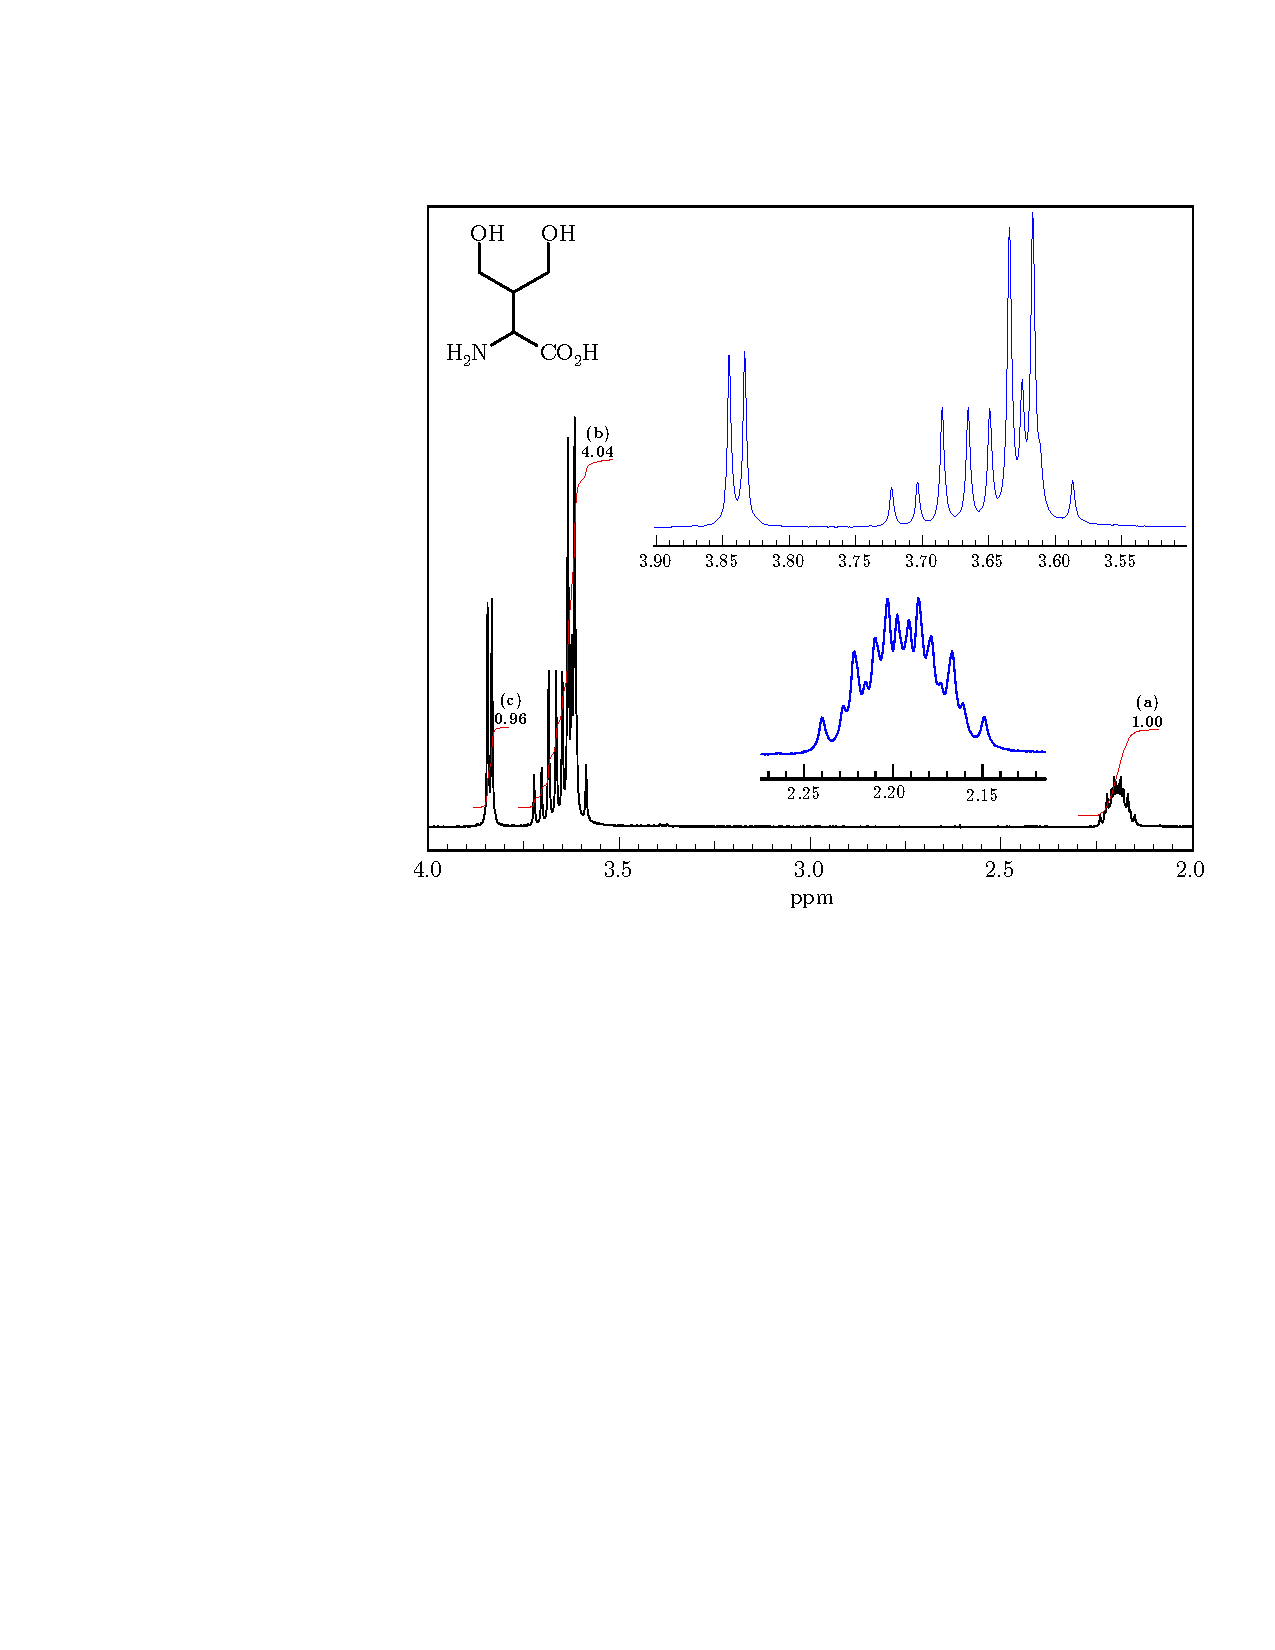
\includegraphics[width=\linewidth]{chimiePC/orga/acideamine.pdf}
    
    Le spectre RMN est effectué dans le $\mathrm{D_2O}$ à 300 MHz.
    
    Nous allons essayer de voir si l'étudiant$\cdot$e a bien synthétisé cette molécule ou non.
\end{EnvUplevel}

\question Identifiez chaque groupe de pics \textbf{(a)}, \textbf{(b)} et \textbf{(c)}.

\question Quels sont les différents couplages possibles ?

\question Calculez le couplage $J_c$ du doublet \textbf{(c)} et commentez sa valeur. \`A quoi correspond ce couplage ?

\question En essayant d'identifier des doublets dans le groupe \textbf{(b)}, attribuez les différents signaux aux couplages associés. On pourra s'aider de l'annexe du handbook.

\end{questions}


\end{exercise}